% !TeX spellcheck = en_US
%Publications.tex
\newcommand{\PublicationsPath}{PatentsAndPublications/Publications}

%PUC 2015

\chapter[A Web-based architecture for multi-device adaptation]{A Web-based distributed architecture for multi-device adaptation in media applications}
\label{chap:PUC2015}
\begin{itemize} \itemsep1pt\parskip0pt\parsep0pt
	\item \textbf{Title:}A Web-based distributed architecture for multi-device adaptation in media applications
	\item \textbf{Authors:} Mikel Zorrilla, Njål Borch, François Daoust, Alexander Erk, Julián Flórez, Alberto Lafuente	
	\item \textbf{Journal:} Personal and Ubiquitous Computing
 	\item \textbf{Publisher:} Springer
	\item \textbf{Year:} 2015
	\item \textbf{DOI:}  \url{http://dx.doi.org/10.1007/s00779-015-0864-x}
\end{itemize}	
	

\ifattachpapers
	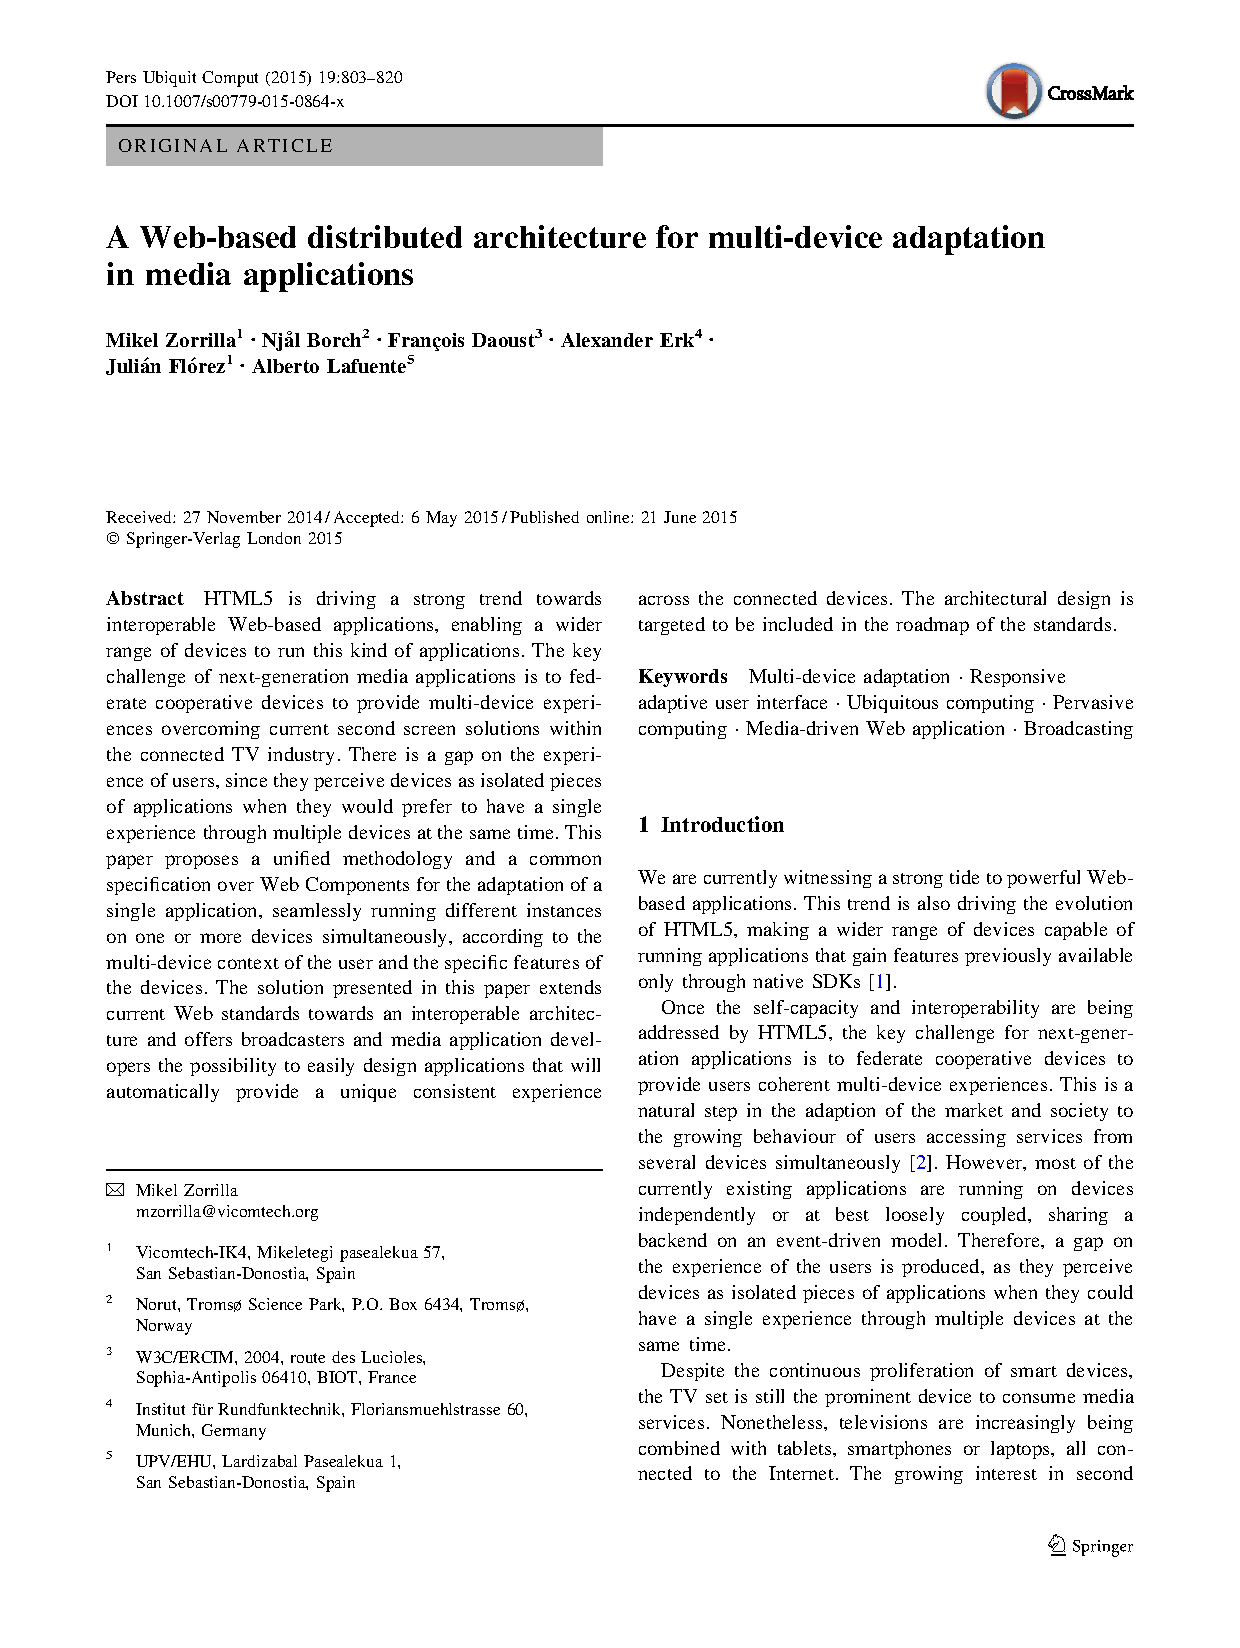
\includepdf[trim=0cm 0cm 0cm -2.2cm,clip,pages=1-last, frame=false, pagecommand={}, nup=1, noautoscale, scale=1, offset = 0.5cm 0cm] {\PublicationsPath/adaptation.pdf}
\fi

%BMSB2015

\chapter[User interface adaptation for multi-device Web-based media]{User interface adaptation for multi-device Web-based media applications}
\label{chap:BMSB2015}
\begin{itemize} \itemsep1pt\parskip0pt\parsep0pt
	\item \textbf{Title:} User interface adaptation for multi-device Web-based media applications
	\item \textbf{Authors:} Mikel Zorrilla, Iñigo Tamayo, Angel Martin, Ana Dominguez	
	\item \textbf{Conference:} Broadband Multimedia Systems and Broadcasting (BMSB)
 	\item \textbf{Publisher:} IEEE
	\item \textbf{Year:} 2015
	\item \textbf{DOI:}  \url{http://dx.doi.org/10.1109/BMSB.2015.7177251}
\end{itemize}	
	

\ifattachpapers
	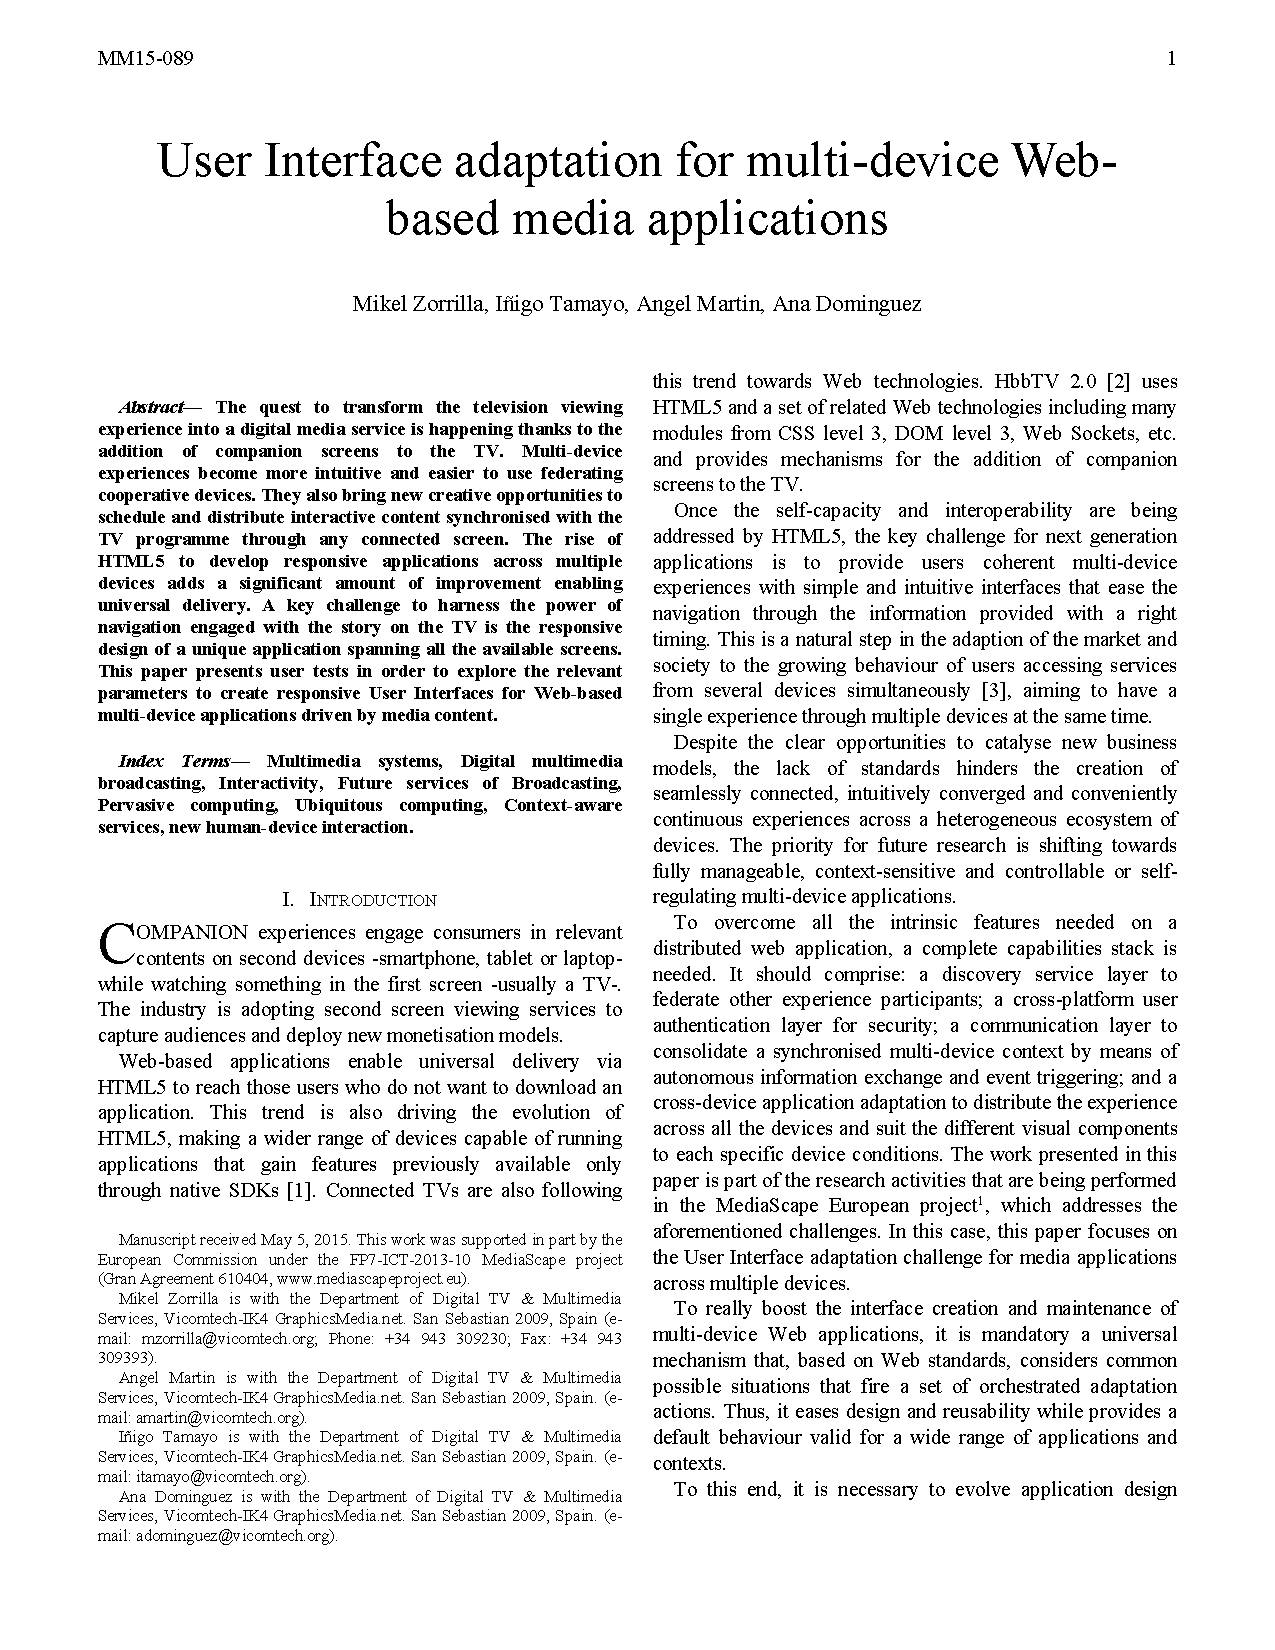
\includepdf[trim=1cm 0cm 0.5cm -1.8cm,clip,pages=1-last, frame=false, pagecommand={}, nup=1, noautoscale, scale=0.98, offset = 0.5cm 0cm] {\PublicationsPath/PID3705461.pdf}
\fi


%BMSB2013

\chapter[Cloud session synchronisation for hbbtv \& mobile devices]{Cloud session maintenance to synchronise hbbtv applications and home network devices}
\label{chap:BMSB2013}
\begin{itemize} \itemsep1pt\parskip0pt\parsep0pt
	\item \textbf{Title:} Cloud session maintenance to synchronise hbbtv applications and home network devices
	\item \textbf{Authors:} Mikel Zorrilla, Iñigo Tamayo, Angel Martin, Igor G Olaizola	
	\item \textbf{Conference:} Broadband Multimedia Systems and Broadcasting (BMSB)
 	\item \textbf{Publisher:} IEEE
	\item \textbf{Year:} 2013
	\item \textbf{DOI:}  \url{http://dx.doi.org/10.1109/BMSB.2013.6621754}
\end{itemize}	
	

\ifattachpapers
	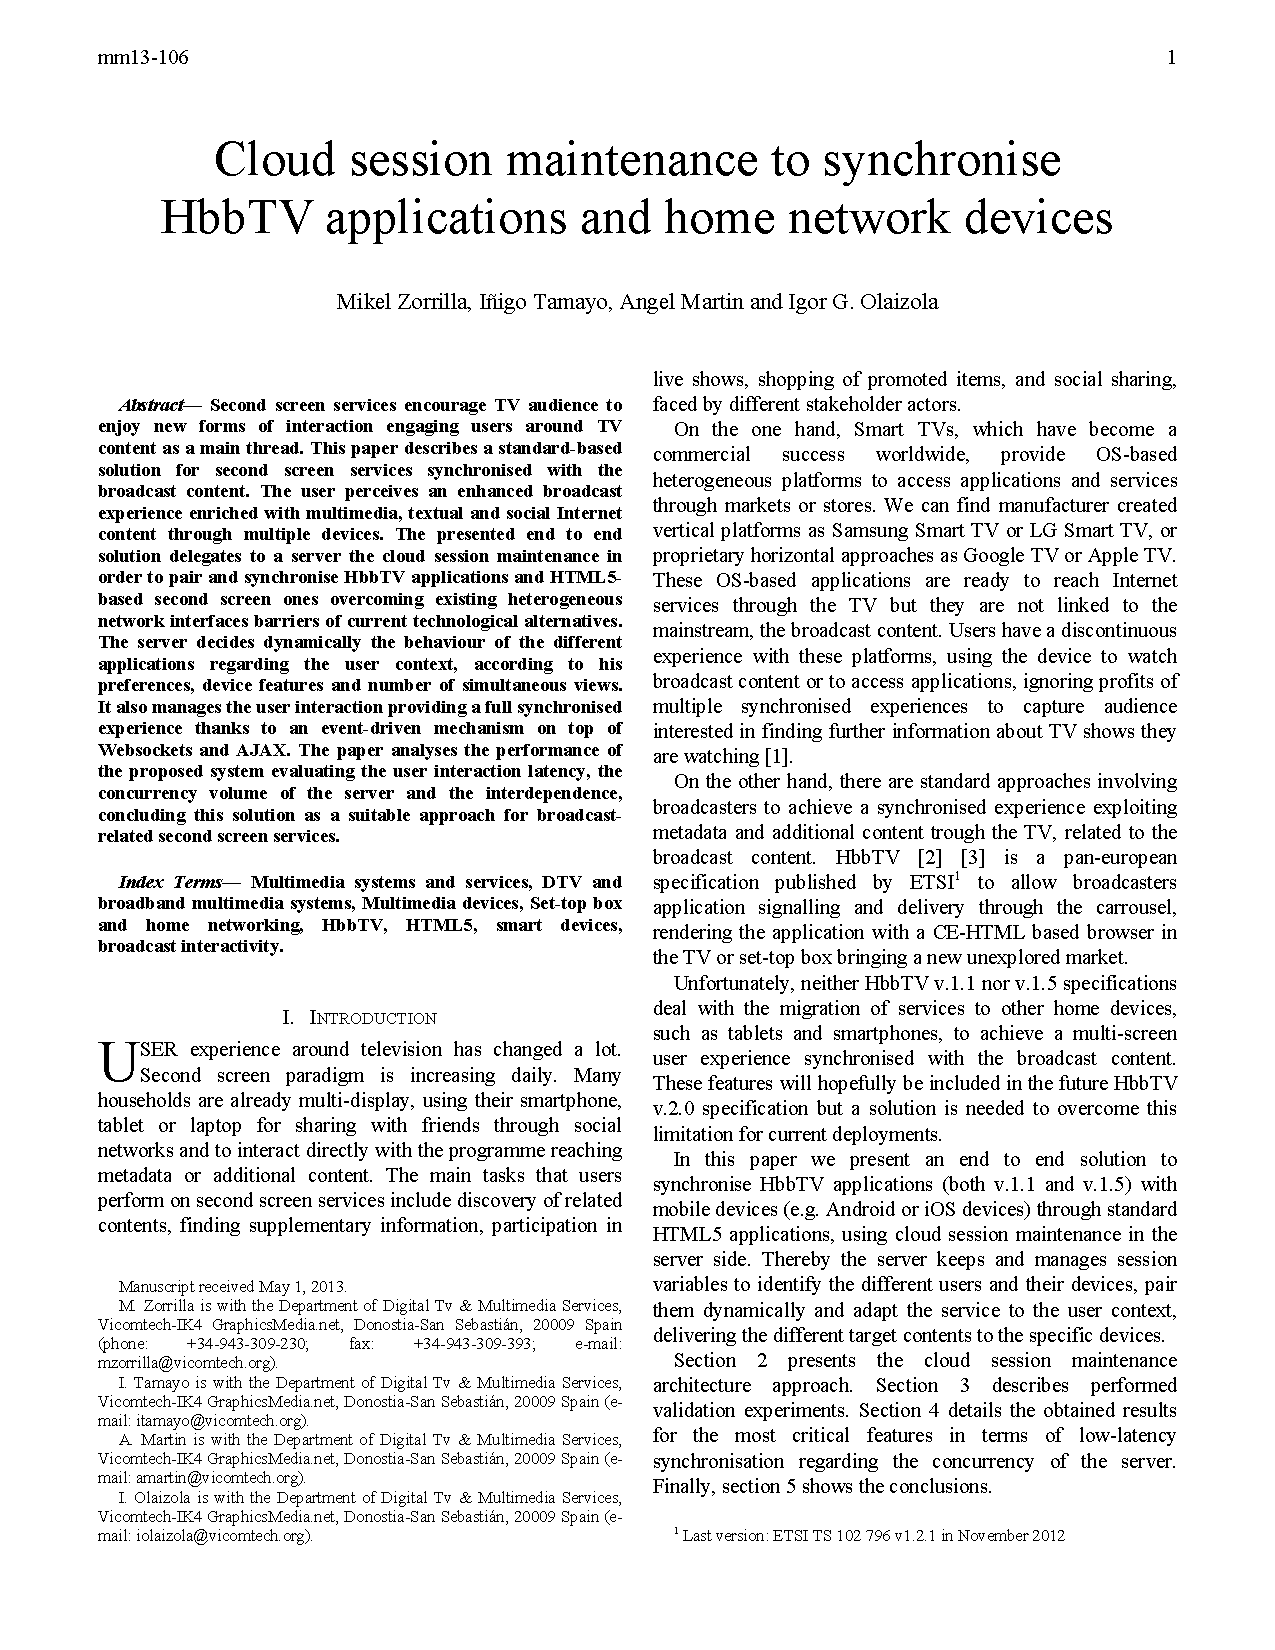
\includepdf[trim=1cm 0cm 0.5cm -2cm,clip,pages=1-last, frame=false, pagecommand={}, nup=1, noautoscale, scale=0.98, offset = 0.5cm 0cm] {\PublicationsPath/PID2766373.pdf}
\fi


%BMSB2014

\chapter[Reaching devices around an HbbTV television]{Reaching devices around an HbbTV television}
\label{chap:BMSB2014}
\begin{itemize} \itemsep1pt\parskip0pt\parsep0pt
	\item \textbf{Title:} Reaching devices around an HbbTV television devices
	\item \textbf{Authors:} Mikel Zorrilla, Angel Martin, Iñigo Tamayo, Sean O'Halpin, Dominique Hazael-Massieux	
	\item \textbf{Conference:} Broadband Multimedia Systems and Broadcasting (BMSB)
 	\item \textbf{Publisher:} IEEE
	\item \textbf{Year:} 2014
	\item \textbf{DOI:}  \url{http://dx.doi.org/10.1109/BMSB.2014.6873499}
\end{itemize}	
	

\ifattachpapers
	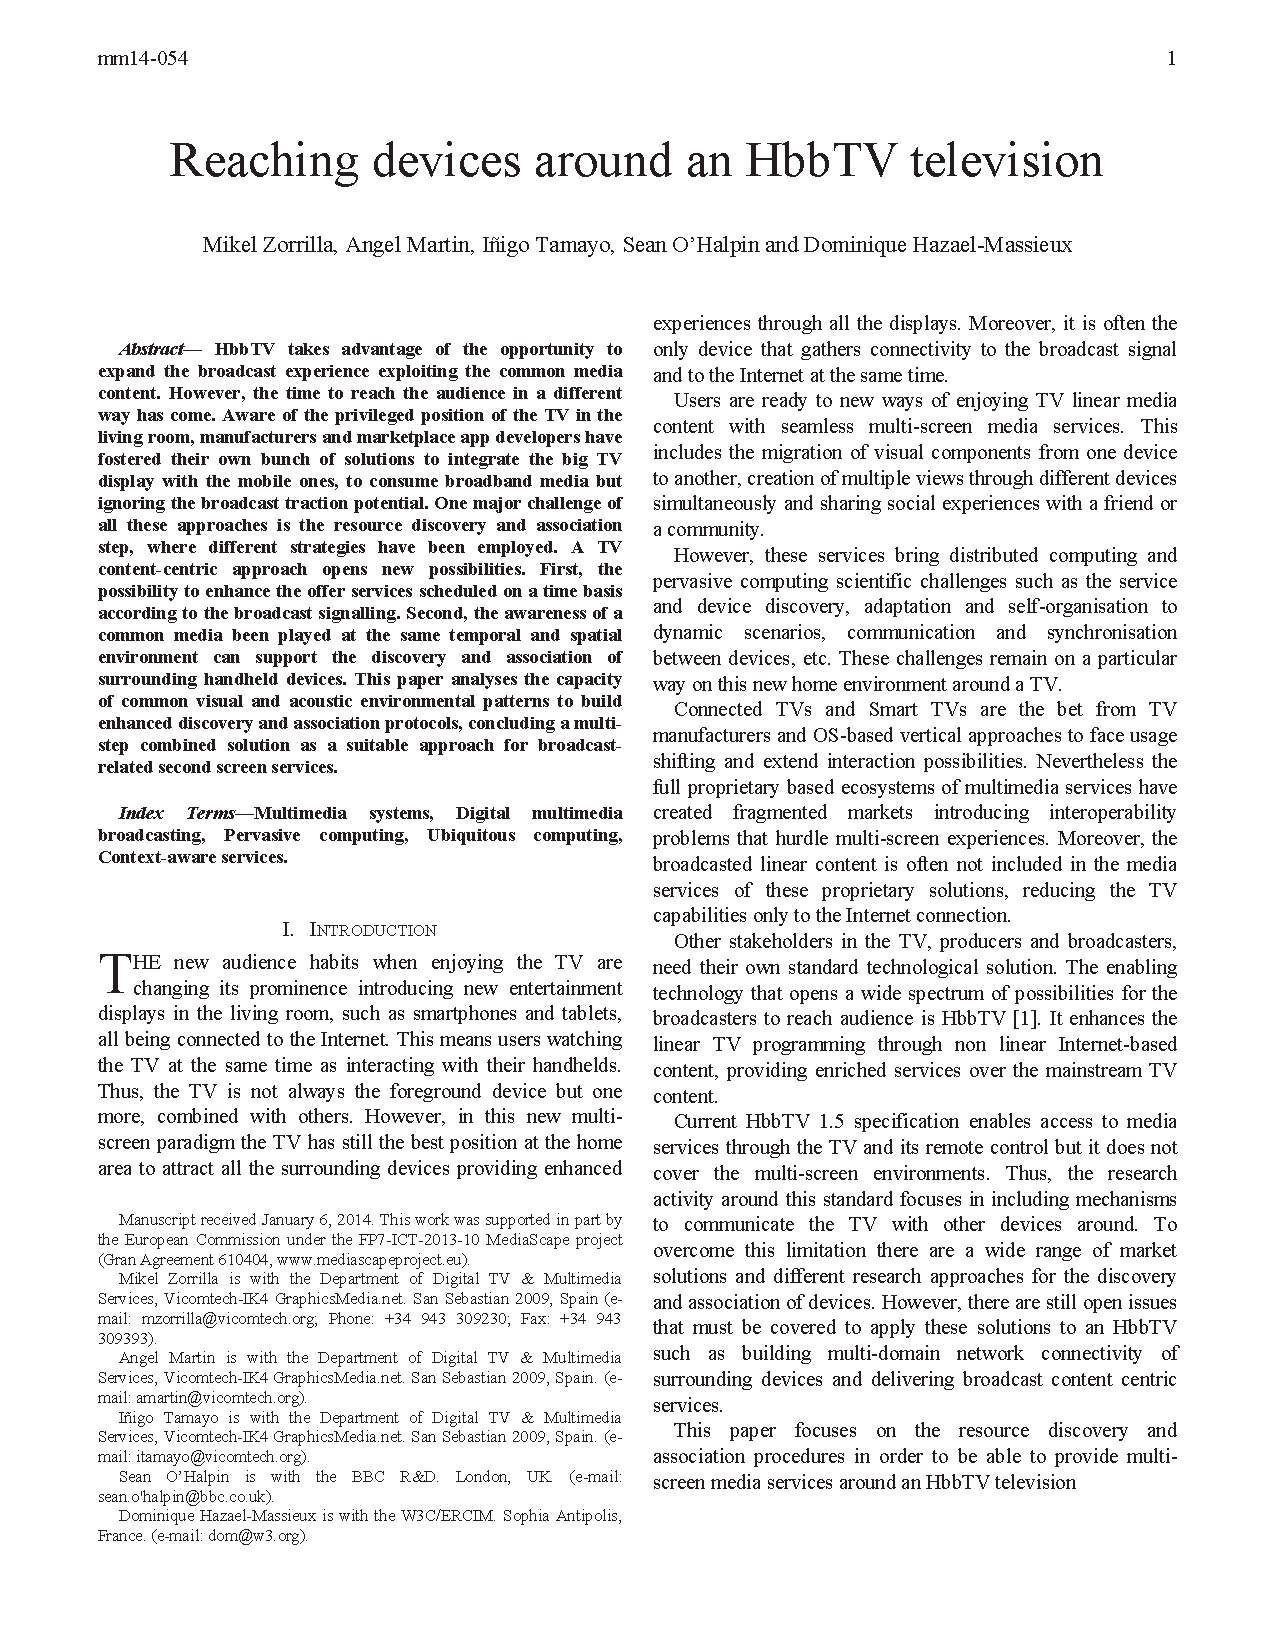
\includepdf[trim=0.8cm 0cm 0.5cm -2cm,clip,pages=1-last, frame=false, pagecommand={}, nup=1, noautoscale, scale=0.97, offset = 0.5cm 0cm] {\PublicationsPath/mm14-054_mzorrilla.pdf}
\fi

%MTAP2014

\chapter[HTML5-based system for interoperable 3D applications]{HTML5-based system for interoperable 3D digital home applications}
\label{chap:MTAP2014}
\begin{itemize} \itemsep1pt\parskip0pt\parsep0pt
	\item \textbf{Title:} HTML5-based system for interoperable 3D digital home applications
	\item \textbf{Authors:} Mikel Zorrilla, Angel Martin, Jairo R. Sanchez, Iñigo Tamayo, Igor G. Olaizola	
	\item \textbf{Conference:} Multimedia Tools and Applications
 	\item \textbf{Publisher:} Springer
	\item \textbf{Year:} 2014
	\item \textbf{DOI:}  \url{http://dx.doi.org/10.1007/s11042-013-1516-7}
\end{itemize}	
	

\ifattachpapers
	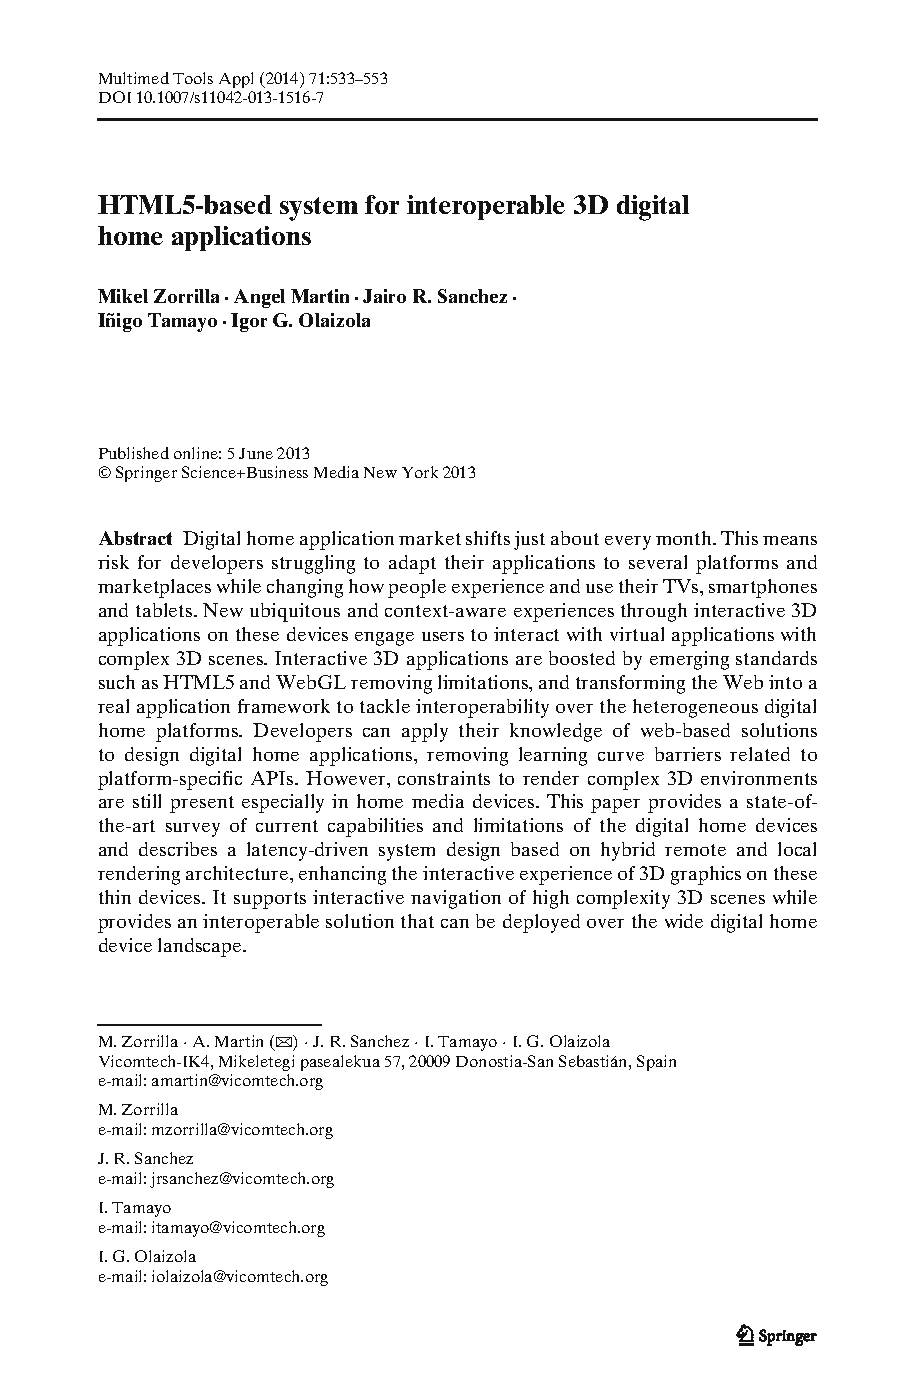
\includepdf[trim=0cm 0cm 0cm -1cm,clip,pages=1-last, frame=false, pagecommand={}, nup=1, noautoscale, scale=1.2, offset = 0.5cm 0cm] {\PublicationsPath/MTAP2014.pdf}
\fi

%TCSVT2016

\chapter[SaW: Video Analysis with Web-based Mobile Grid Computing]{SaW: Video Analysis in Social Media with Web-based Mobile Grid Computing}
\label{chap:TCSVT2016}
\begin{itemize} \itemsep1pt\parskip0pt\parsep0pt
	\item \textbf{Title:} SaW: Video Analysis in Social Media with Web-based Mobile Grid Computing
	\item \textbf{Authors:} Mikel Zorrilla, Julián Flórez, Alberto Lafuente, Angel Martin, Igor G. Olaizola, Iñigo Tamayo	
	\item \textbf{Conference:} Transactions on Circuits and Systems for Video Technology
 	\item \textbf{Publisher:} IEEE
	\item \textbf{Year:} 2016
\end{itemize}	
	

\ifattachpapers
	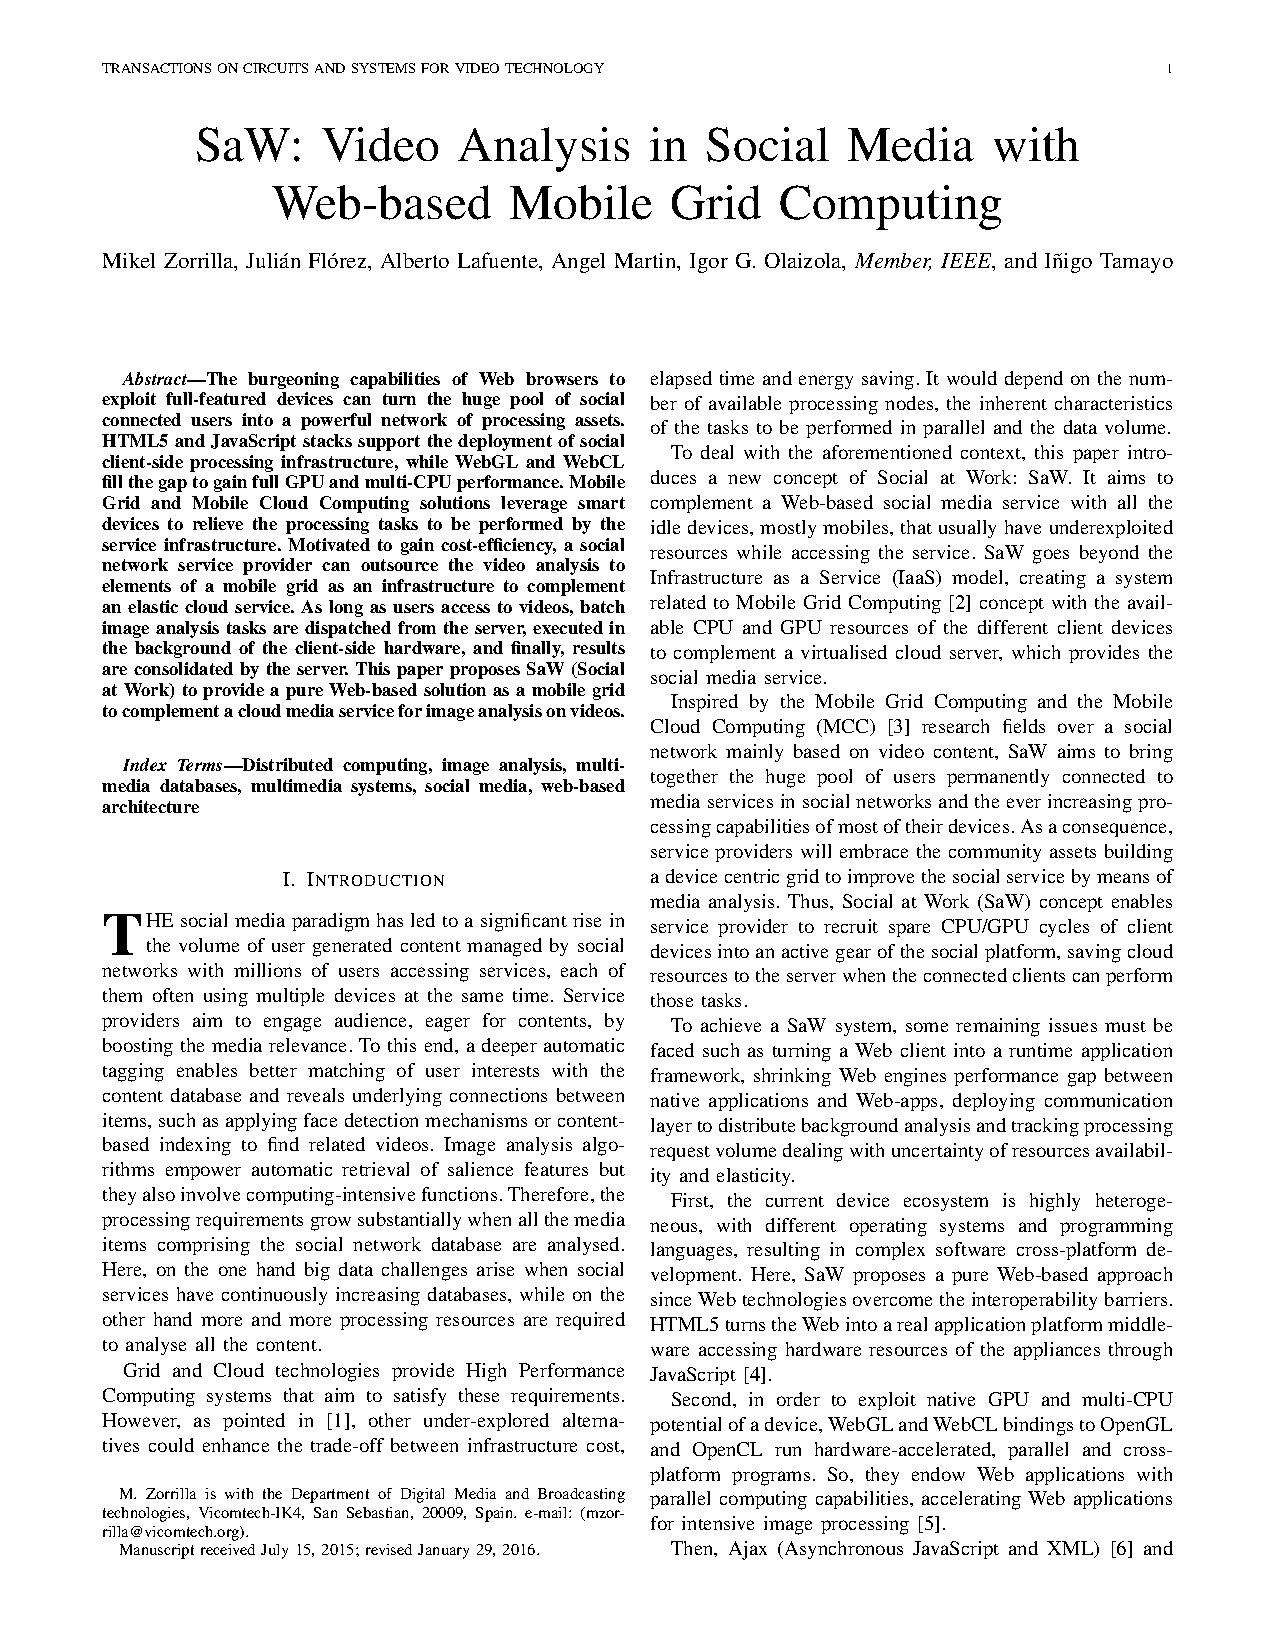
\includepdf[trim=1cm 0cm 0.5cm -1.4cm,clip,pages=1-14, frame=false, pagecommand={}, nup=1, noautoscale, scale=0.97, offset = 0.5cm 0cm] {\PublicationsPath/SaW_final_20160129.pdf}
\fi

\chapter{Author's other publications}

List of other publications:

\begin{enumerate}
\item 
\begin{itemize} \itemsep1pt\parskip0pt\parsep0pt
	\item \textbf{Title:} Web Browser-Based Social Distributed Computing Platform Applied to Image Analysis
	\item \textbf{Authors:} Mikel Zorrilla, Angel Martin, Iñigo Tamayo, Naiara Aginako, Igor G. Olaizola
	\item \textbf{Proceedings:} Cloud and Green Computing (CGC)
	\item \textbf{Pages:} 389-396
 	\item \textbf{Publisher:} IEEE
	\item \textbf{Year:} 2013
	\item \textbf{DOI:} \url{http://dx.doi.org/10.1109/CGC.2013.68}
	\item \textbf{Abstract:} \textit{In this paper we introduce a new platform to perform image processing algorithms over big data. The main stakeholders of media analysis are the social services which manage huge volumes of multimedia data. While social service providers have already a big resources pool of connected assets through the devices of the community, they are not exploiting them for their processing needs and they usually deploy high performance systems that run batch works. Image processing requires parallelizable atomic and lightweight tasks that can benefit from a big community of thin devices executing seamless background processes while the user enjoys other social media contents. To provide such infrastructure a client-side browser solution based on JavaScript libraries has been developed. We also describe a performance model that establishes the contexts where the solution gets ahead in terms of available resources and the processing problem nature.}
\end{itemize}
\hrulefill
\item 
\begin{itemize} \itemsep1pt\parskip0pt\parsep0pt
	\item \textbf{Title:} Reference Model for Hybrid Broadcast Web3D TV
	\item \textbf{Authors:} Igor García Olaizola, Josu Pérez, Mikel Zorrilla, Angel Martin, Maider Laka
	\item \textbf{Proceedings:} 3D Web Technology (Web3D)
	\item \textbf{Pages:} 177-180
 	\item \textbf{Publisher:} ACM
	\item \textbf{Year:} 2013
	\item \textbf{DOI:} \url{http://dx.doi.org/10.1145/2466533.2466560}
	\item \textbf{Abstract:} \textit{3DTV can be considered as the biggest technical revolution in TV content creation since the black and white to color transition. However, the big commercial success of current TV market has been produced around the Smart TV concept. Smart TVs connect the TV set to the web and introduce the main home multimedia display in the app world, social networks and content related interactive services. Now, this digital convergence can become the driver for boosting the success of 3DTV industry. In fact, the integration of stereoscopic TV production and Web3D seems to be the next natural step of the hybrid broadband-broadcast services. We propose in this paper a general reference model to allow the convergence of 3DTV and 3D Web by defining a general architecture and some extensions of current Smart TV concepts as well as the related standards.}
\end{itemize}
\hrulefill
\item 
\begin{itemize} \itemsep1pt\parskip0pt\parsep0pt
	\item \textbf{Title:} HTML5-based System for Interoperable 3D Digital Home Applications
	\item \textbf{Authors:} Mikel Zorrilla, Angel Martin, Jairo R. Sanchez, Iñigo Tamayo, Igor G. Olaizola
	\item \textbf{Proceedings:} Digital Home (ICDH)
	\item \textbf{Pages:} 206-214
 	\item \textbf{Publisher:} IEEE
	\item \textbf{Year:} 2012
	\item \textbf{DOI:} \url{http://dx.doi.org/10.1109/ICDH.2012.21}
	\item \textbf{Abstract:} \textit{Digital home application market shifts just about every month. This means risk for developers struggling to adapt their applications to several platforms and marketplaces while changing how people experience and use their TVs, smartphones and tablets. New ubiquitous and context-aware experiences through interactive 3D applications on these devices engage users to interact with complex 3D scenes in virtual applications. Interactive 3D applications are boosted by emerging standards such as HTML5 and WebGL removing limitations, and transforming the Web into a horizontal application framework to tackle interoperability over the heterogeneous digital home platforms. Developers can apply their knowledge of web-based solutions to design digital home applications, removing learning curve barriers related to platform-specific APIs. However, constraints to render complex 3D environments are still present especially in home media devices. This paper provides a state-of-the-art survey of current capabilities and limitations of the digital home devices and describes a latency-driven system design based on hybrid remote and local rendering architecture, enhancing the interactive experience of 3D graphics on these thin devices. It supports interactive navigation of sophisticated 3D scenes while provides an interoperable solution that can be deployed over the wide digital home device landscape.}
\end{itemize}
\hrulefill
\item 
\begin{itemize} \itemsep1pt\parskip0pt\parsep0pt
	\item \textbf{Title:} End to end solution for interactive on demand 3d media on home network devices
	\item \textbf{Authors:} Mikel Zorrilla, Angel Martin, Felipe Mogollon, Julen García, Igor G. Olaizola
	\item \textbf{Proceedings:} Broadband Multimedia Systems and Broadcasting (BMSB)
	\item \textbf{Pages:} 1-6
 	\item \textbf{Publisher:} IEEE
	\item \textbf{Year:} 2012
	\item \textbf{DOI:} \url{http://dx.doi.org/10.1109/BMSB.2012.6264228}
	\item \textbf{Abstract:} \textit{Smart devices have deeply modified the user consumption expectations getting used to rich interactive experiences around new media services. In this emerging landscape, TV rises as the central media device integrating the home network ecosystem. In the race to create more dynamic and customizable content, computer generated 3D graphics get a prominent position combined with video and audio to provide immersive and realistic environments in advanced applications where the user interaction is crucial. However, current home devices lack the required specific hardware to perform it. The proposed 3DMaaS System faces this scenario by performing 3D cloud rendering through streaming sessions with each client device, taking benefit of the Internet connectivity and video streaming management capabilities that most of thin devices have. In order to deal with the wide spectrum of device features, 3DMaaS provides a complete set of streaming formats, including RTSP, HLS and MPEG-DASH, that also fits new trends in media consumption brought by HTML5 and HbbTV. This paper presents latency performance profiling over the different streaming protocols which have a direct influence on the user interaction experience.}
\end{itemize}
\hrulefill
\item 
\begin{itemize} \itemsep1pt\parskip0pt\parsep0pt
	\item \textbf{Title:} HBB4ALL: Deployment of HbbTV services for all
	\item \textbf{Authors:} Pilar Orero, Carlos A. Martín, Mikel Zorrilla
	\item \textbf{Proceedings:} Broadband Multimedia Systems and Broadcasting (BMSB)
	\item \textbf{Pages:} 1-4
 	\item \textbf{Publisher:} IEEE
	\item \textbf{Year:} 2015
	\item \textbf{DOI:} \url{http://dx.doi.org/10.1109/BMSB.2015.7177252}
	\item \textbf{Abstract:} \textit{Hybrid Broadcast Television for All is a European Commission co-financed project, inside the Competitiveness and Innovation Framework Programme (CIP). The project builds on HbbTV, the European standard for broadcast and broadband multimedia converged services, and looks at how HbbTV technology may be used to enhance access services (such as subtitling, audio description or sign language) on both the production and service sides. HbbTV 1.5 devices are widely available in the market while HbbTV version 2.0 specification has been recently released. TV content can be enhanced by HbbTV applications with additional synchronised services in a personalised manner. For access services this opens an entirely new opportunity for users who may choose an access service delivered via their IP connection which seamlessly integrates with the regular broadcast programme. The presentation will describe the improvements taken on board by HBB4ALL to existing access services and ways of addressing the key technical, organisational and legal obstacles to the sustainable take-up of these services throughout Europe. HBB4ALL focuses on real pilot deployment as a first step to ensure a successful exploitation of these services in a near future. We will offer new insights, from the fields of human machine interaction and social innovation, which arise from the new interactive multimodal and multilanguage services which may be offered. This article will first describe the structure chosen for the project, with four pilots developed in parallel: subtitling, audio description, sign language and user interaction. Then it will describe the methodology and research approaches used for testing the new accessibility services.}
\end{itemize}
\hrulefill
\item 
\begin{itemize} \itemsep1pt\parskip0pt\parsep0pt
	\item \textbf{Title:} Ontology-based tourism for all recommender and information retrieval system for interactive community displays
	\item \textbf{Authors:} Kevin Alonso, Mikel Zorrilla, Roberto Confalonieri, Javier Vazquez-Salceda, Hasier Iñan, Manel Palau, Javier Calle, Elena Castro
	\item \textbf{Proceedings:} Information Science and Digital Content Technology (ICIDT)
	\item \textbf{Pages:} 650-655
 	\item \textbf{Publisher:} IEEE
	\item \textbf{Year:} 2012
	\item \textbf{Abstract:} \textit{This paper presents a multi-stage ontology-based touristic recommender system which offers: personalized suggestions to citizens and tourists, including those with special needs; and information concerning the suggested locations. The system's suggestions are based on user profiles which are continuously updated via feedback obtained from past interactions. Users' preferences are deducted by means of profiles and they are used to create and to send queries to heterogeneous information sources. The results are ranked and presented to the user along with related information.}
\end{itemize}
\hrulefill
\item 
\begin{itemize} \itemsep1pt\parskip0pt\parsep0pt
	\item \textbf{Title:} Next Generation Multimedia on Mobile Devices
	\item \textbf{Authors:} Mikel Zorrilla, M. del Puy Carretero, Alex Ugarte, Felipe Mogollon, David Oyarzun, Igor G. Olaizola
	\item \textbf{Article:} Mobile Technology Consumption: Opportunities and Challenges: Opportunities and Challenges
	\item \textbf{Pages:} 168
 	\item \textbf{Publisher:} IGI Global
	\item \textbf{Year:} 2011
	\item \textbf{Abstract:} \textit{The multiplatform consumption of multimedia content has become a crucial factor in the way of watching multimedia. Current technologies such as mobile devices have made people desire access to information from anywhere and at anytime. The sources of the multimedia content are also very important in that consumption. They present the content from many sources distributed on the cloud and mix it with automatically generated virtual reality into any platform. This chapter analyzes the technologies to consume the next generation multimedia and proposes a new architecture to generate and present the content. The goal is to offer it as a service so the users can live the experience in any platform, without requiring any special abilities from the clients. This makes the architecture a very interesting aspect for mobile devices that normally do not have big capabilities of rendering but can benefit of this architecture.}
\end{itemize}
\hrulefill

\end{enumerate}

